\section{Numerical  experiments}

\paragraph*{Simulation study.} We propose a simple simulation to
illustrate the interest of using multiattribute networks.  The
simulations are set up as follows:
\begin{enumerate}
\item  Draw  a random  undirected  network  with  $p$ nodes  from  the
  Erd\"os-Renyi model with adajacency matrix $\bA$;
\item  Expand the  associated adjacency  matrix to  multivariate space
  with
  $$\mathbf{M} = \mathbf{A}  \otimes \mathbb{S} + \mathbf{I}_{p\times K}$$
  where $\otimes$ is the Kronecker product. The $K\times K$ matrix
  $\mathbb{S}$ is used to consider different scenarios of agreement
  across the attributes of two genes. We consider three cases
  \begin{enumerate}
  \item $\mathbb{S} = \mathbf{I}_{K,K}$ the $K\times K$ identity
    matrix: same intra-attribute network and no inter-attribute
    interactions;
  \item $\mathbb{S} = \mathbf{I}_{K,K} - \mathbf{1}_{K,K}$, same
    inter-attribute interactions and no intra-attribute interactions;
  \item $\mathbb{S} = \mathbf{1}_{K,K}$ a matrix full of one: full
    agreement between  attributes.
  \end{enumerate}
\item Compute $\bTheta$ a positive definite approximation of
  $\mathbf{M}$ by replacing null and negative eigenvalues by a small constant;
\item Control the difficulty of  the problem with $\gamma>0$ such that
  $\bTheta= \bTheta+ \gamma I$;
\item Draw an i.i.d. $n$-size sample $\bX\in\Rset^{n\times pK}$ of
  $X \sim \mathcal{N} \left( 0,\invcov^{-1} \right) .$
\end{enumerate}

We choose small networks with $p=40$, with $40$ edges on average and
vary $n$ from $p/2$ to $2p$. We fix $\gamma$ to $0.1$ and consider
cases where the number of attributes is $K=2,3$ and $4$. We compare
our multiattribute approach of neighborhood selection to two
baselines:
\begin{enumerate}
\item the standard neighborhood selection procedure applied on the
  data related to each attribute separately: to do so, we separate
  $\bX$ in $K$ data sets $\bX^{(1)}, \dots \bX^{(K)}$ all with size
  $\Rset^{n\times p}$ and reconstruct one network per attribute. We
  refer to this method as the \textit{separate} variant.
\item the standard neighborhood selection approach applied on a merge
  data set, obtained by stacking the data sets
  $\bX^{(1)}, \dots \bX^{(K)}$ of each attribute into a single
  $\tilde\bX$ data set in $\Rset^{nK \times p}$. We refer to this
  method as the \textit{merge} variant. This method is the exact
  opposite of the \textit{separate} variant.
\end{enumerate}
We assess the performances of each method in reconstructing the
original adjacency matrix $\bA$ with the area under ROC curve
(AUC). For the \textit{separate} variant, the retained AUC is the AUC
averaged over all attributes. We replicate the experiment 100 times.

On Figure \ref{fig:simu_multi}, it is clear that aggregation (either
by merging data sets or with multiattribute network inference)
improves upon a single-attribute approach. Even when there is no
inter-attributes interactions, (which is barely meaningful towards
application to regulatory networks), in which case it is a very good
idea to merge the problems together to increase the sample size, our
multiattribute approach remains quite competitive and robust. In all
other cases, it outperforms the competing approaches.
\begin{figure}[htbp!]
  \centering
  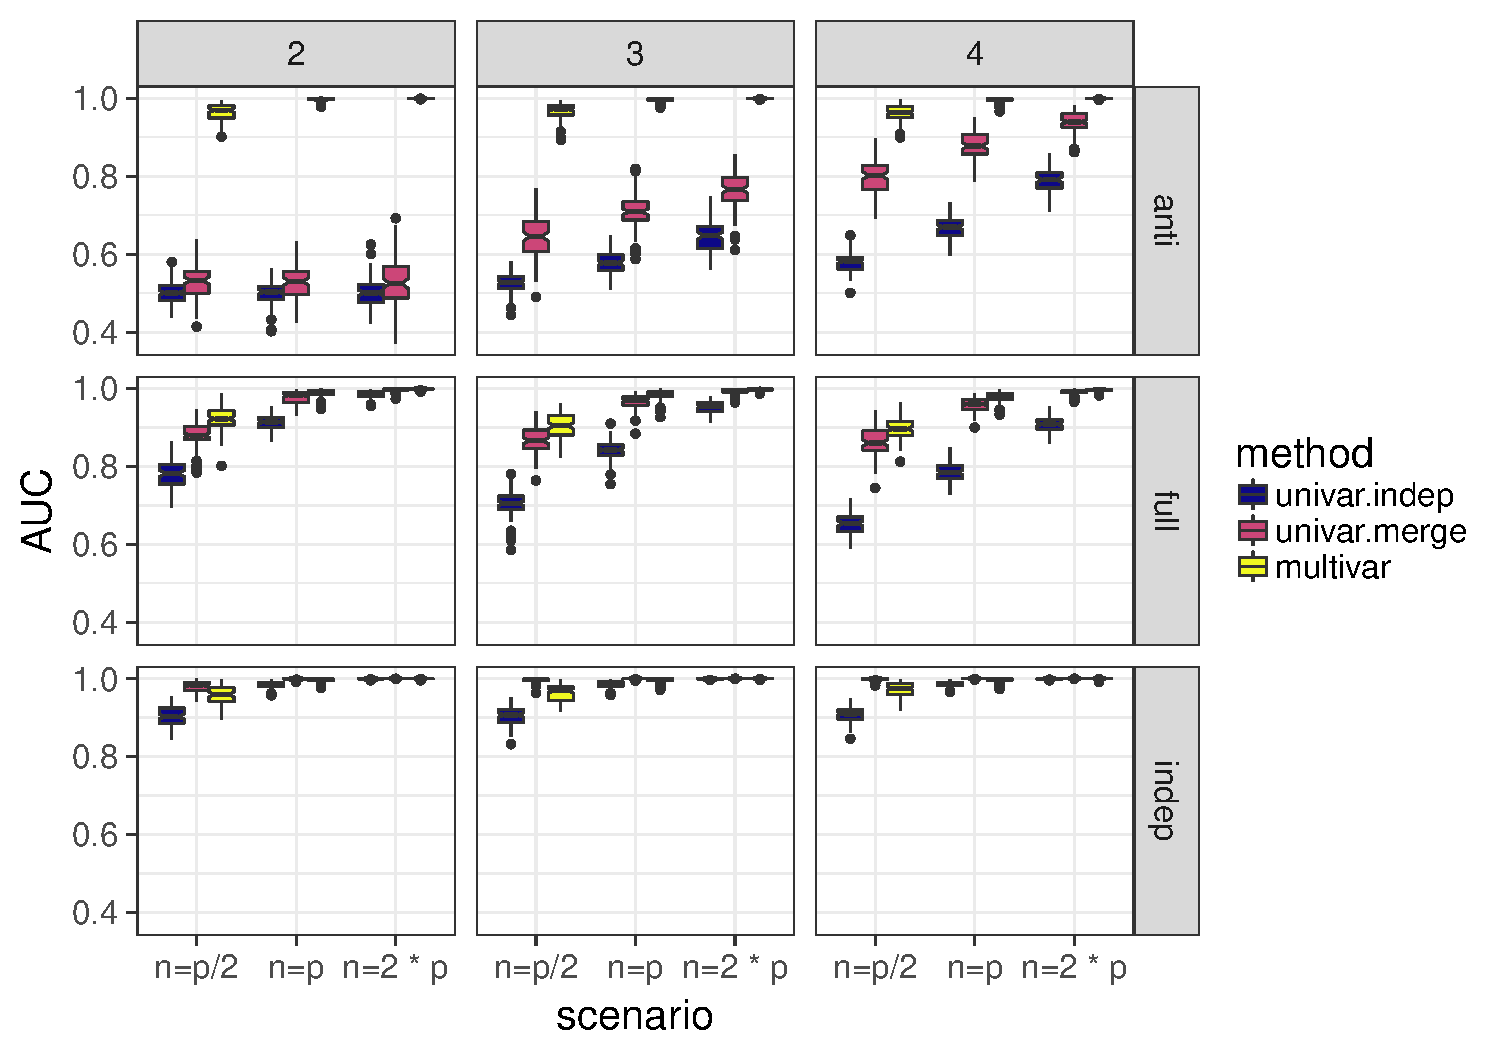
\includegraphics[width=\textwidth]{figures/res_simu_new}
  \caption{Simple simulation study for the multiattribute network
    inference problem: the multiattribute procedure improves over the
    univariate procedures in every situation when networks are close
    for each attribute.}
  \label{fig:simu_multi}
\end{figure}
